\documentclass{article}
\usepackage[utf8]{inputenc}

\usepackage[T2A]{fontenc}
\usepackage[utf8]{inputenc}
\usepackage[russian]{babel}

\usepackage{amsmath}
\usepackage{graphicx}

\title{Вычислительная техника}
\author{Лисид Лаконский}
\date{October 2022}

\begin{document}

\maketitle
\tableofcontents
\pagebreak

\section{Вычислительная техника - 03.10.2022}

Ревью прошлого зантия: совершенная дизъюнктивная (или) форма, соершенная конъюнктивная (и) нормальная форма, минимазция с помощью трех методов: алгебраического, с помощью карт Карно, с помощью диаграммы Вейча.

\subsection{Табличные методы минимизации}

\subsubsection{Минимизация с помощью карт Карно}

$
\begin{pmatrix}
     & 0 & 1 \\
    0 \\
    1
\end{pmatrix}
$ - шаблон карты Карно для функции, принимающей два аргумента.

$
\begin{pmatrix}
     & 00 & 01 & 11 & 10 \\
    0 \\
    1
\end{pmatrix}
$ - шаблон карты Карно для функции, принимающей три аргумента.

$
\begin{pmatrix}
     & 00 & 01 & 11 & 10 \\
    00 \\
    01 \\
    11 \\
    10
\end{pmatrix}
$ - шаблон карты Карно для функции, принимающей четыре аргумента.

Основные принципы склейки:

\begin{enumerate}
    \item Склейку клеток одной и той же карты Карно можно осуществлять как по единицам (a), так и по нулям (б). Первое необходимо для получения ДНФ, второе — для получения КНФ
    \item Склеивать можно только прямоугольные области с числом единиц (нулей), являющимся целой степенью двойки
    \item Рекомендуется выбирать максимально возможные области склейки
    \item Для карт Карно с числом переменных 3 и 4 применимо следующее правило: крайние клетки каждой горизонтали и каждой вертикали граничат между собой и могут объединяться в прямоугольники (топологически карта Карно представляет собой тор). Следствием этого правила является смежность всех четырёх угловых ячеек карты Карно для 4 переменных
\end{enumerate}

\subsubsection{Минимизация с помощью диаграмм Вейча}

Метод минимизации с помощью диаграмм Вейча основан на методе с применением карт Карно, однако элементы записываются иначе, более удобно для формирования итоговой формулы: лучше смотреть, что изменяется, а что нет.

Все записывается так же с помощью кода Грея, неизменяющиеся элементы подписываются так, чтобы образовывать единицу.

\subsection{Цифровые комбинационные устройства}

\subsubsection{Устройство равнозначности}

$y = (x_{1}x_{2}) + (\overline{x_{1}}\overline{x_{2}}) = \overline{\overline{x_{1}x_{2}} * \overline{\overline{x_1}\overline{x_2}}}$

Возвращает единицу, если оба аргумента равны, иначе ноль.

\subsubsection{Устройство неравнозначности}

$y = x_1\overline{x_2} + \overline{x_1}x_2$

Возвращает единицу, если оба аргумента не равны, иначе ноль.

\subsubsection{Полусумматор}

$S = x_1 \oplus x_2, P = x_{1}x_{2}$

$S$ - сумма, $P$ - перенос

\subsubsection{Комбинационный сумматор}

Комбинационный сумматор, удивительно, получается при помощии комбинации полусумматоров или других сумматоров.

Схемы тут не будет, так как в LaTeX крайне неудобно прикреплять картинки. По крайней мере, мне лень сейчас разбираться, как тут в Overleaf это делать.

Складываются аргументы, а потом результат работы сумматора складывается с переносом.

\pagebreak
\section{Вычислительная техника - 17.10.2022}

\subsection{Шифраторы}

\begin{flushleft}

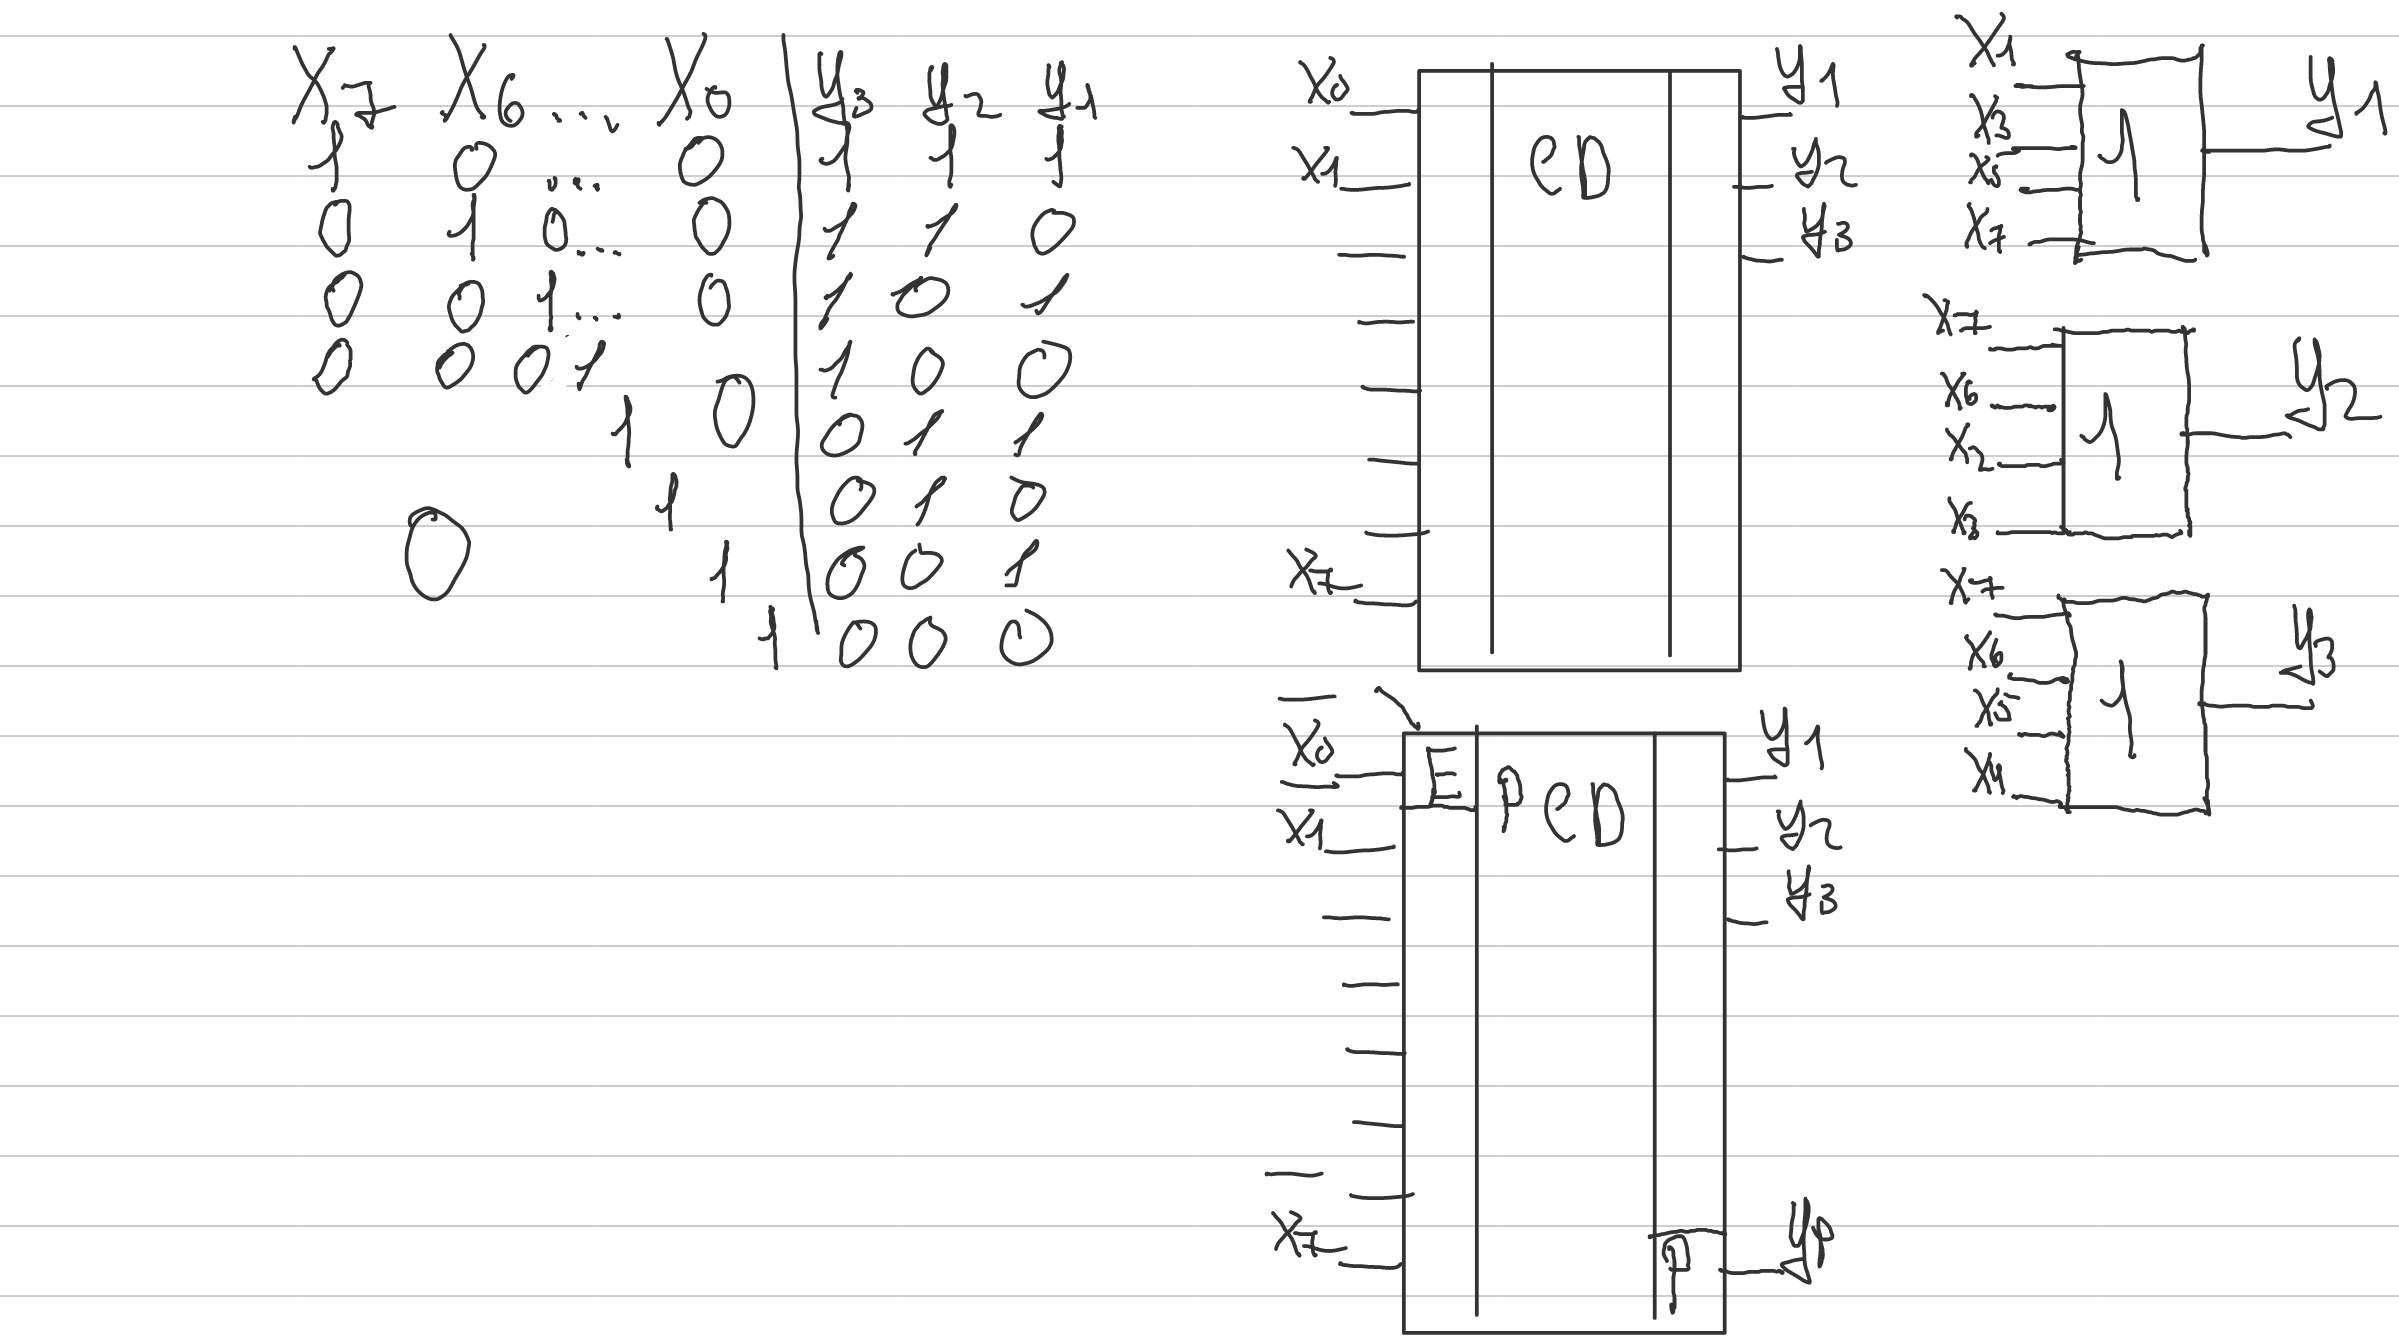
\includegraphics[width=\textwidth]{assets/coder.png}

\subsubsection{Устранение неоднозначности}

Устранять неоднозначность можно с помощью приоритетного шифратора - дополнительный выход $p$ - выход признака невозбуждения: 0 - возбужден хотя бы один из входов, 1 - в противном случае, дополнительный вход $E$.

\subsection{Дешифраторы}

\subsubsection{Линейные дешифраторы}

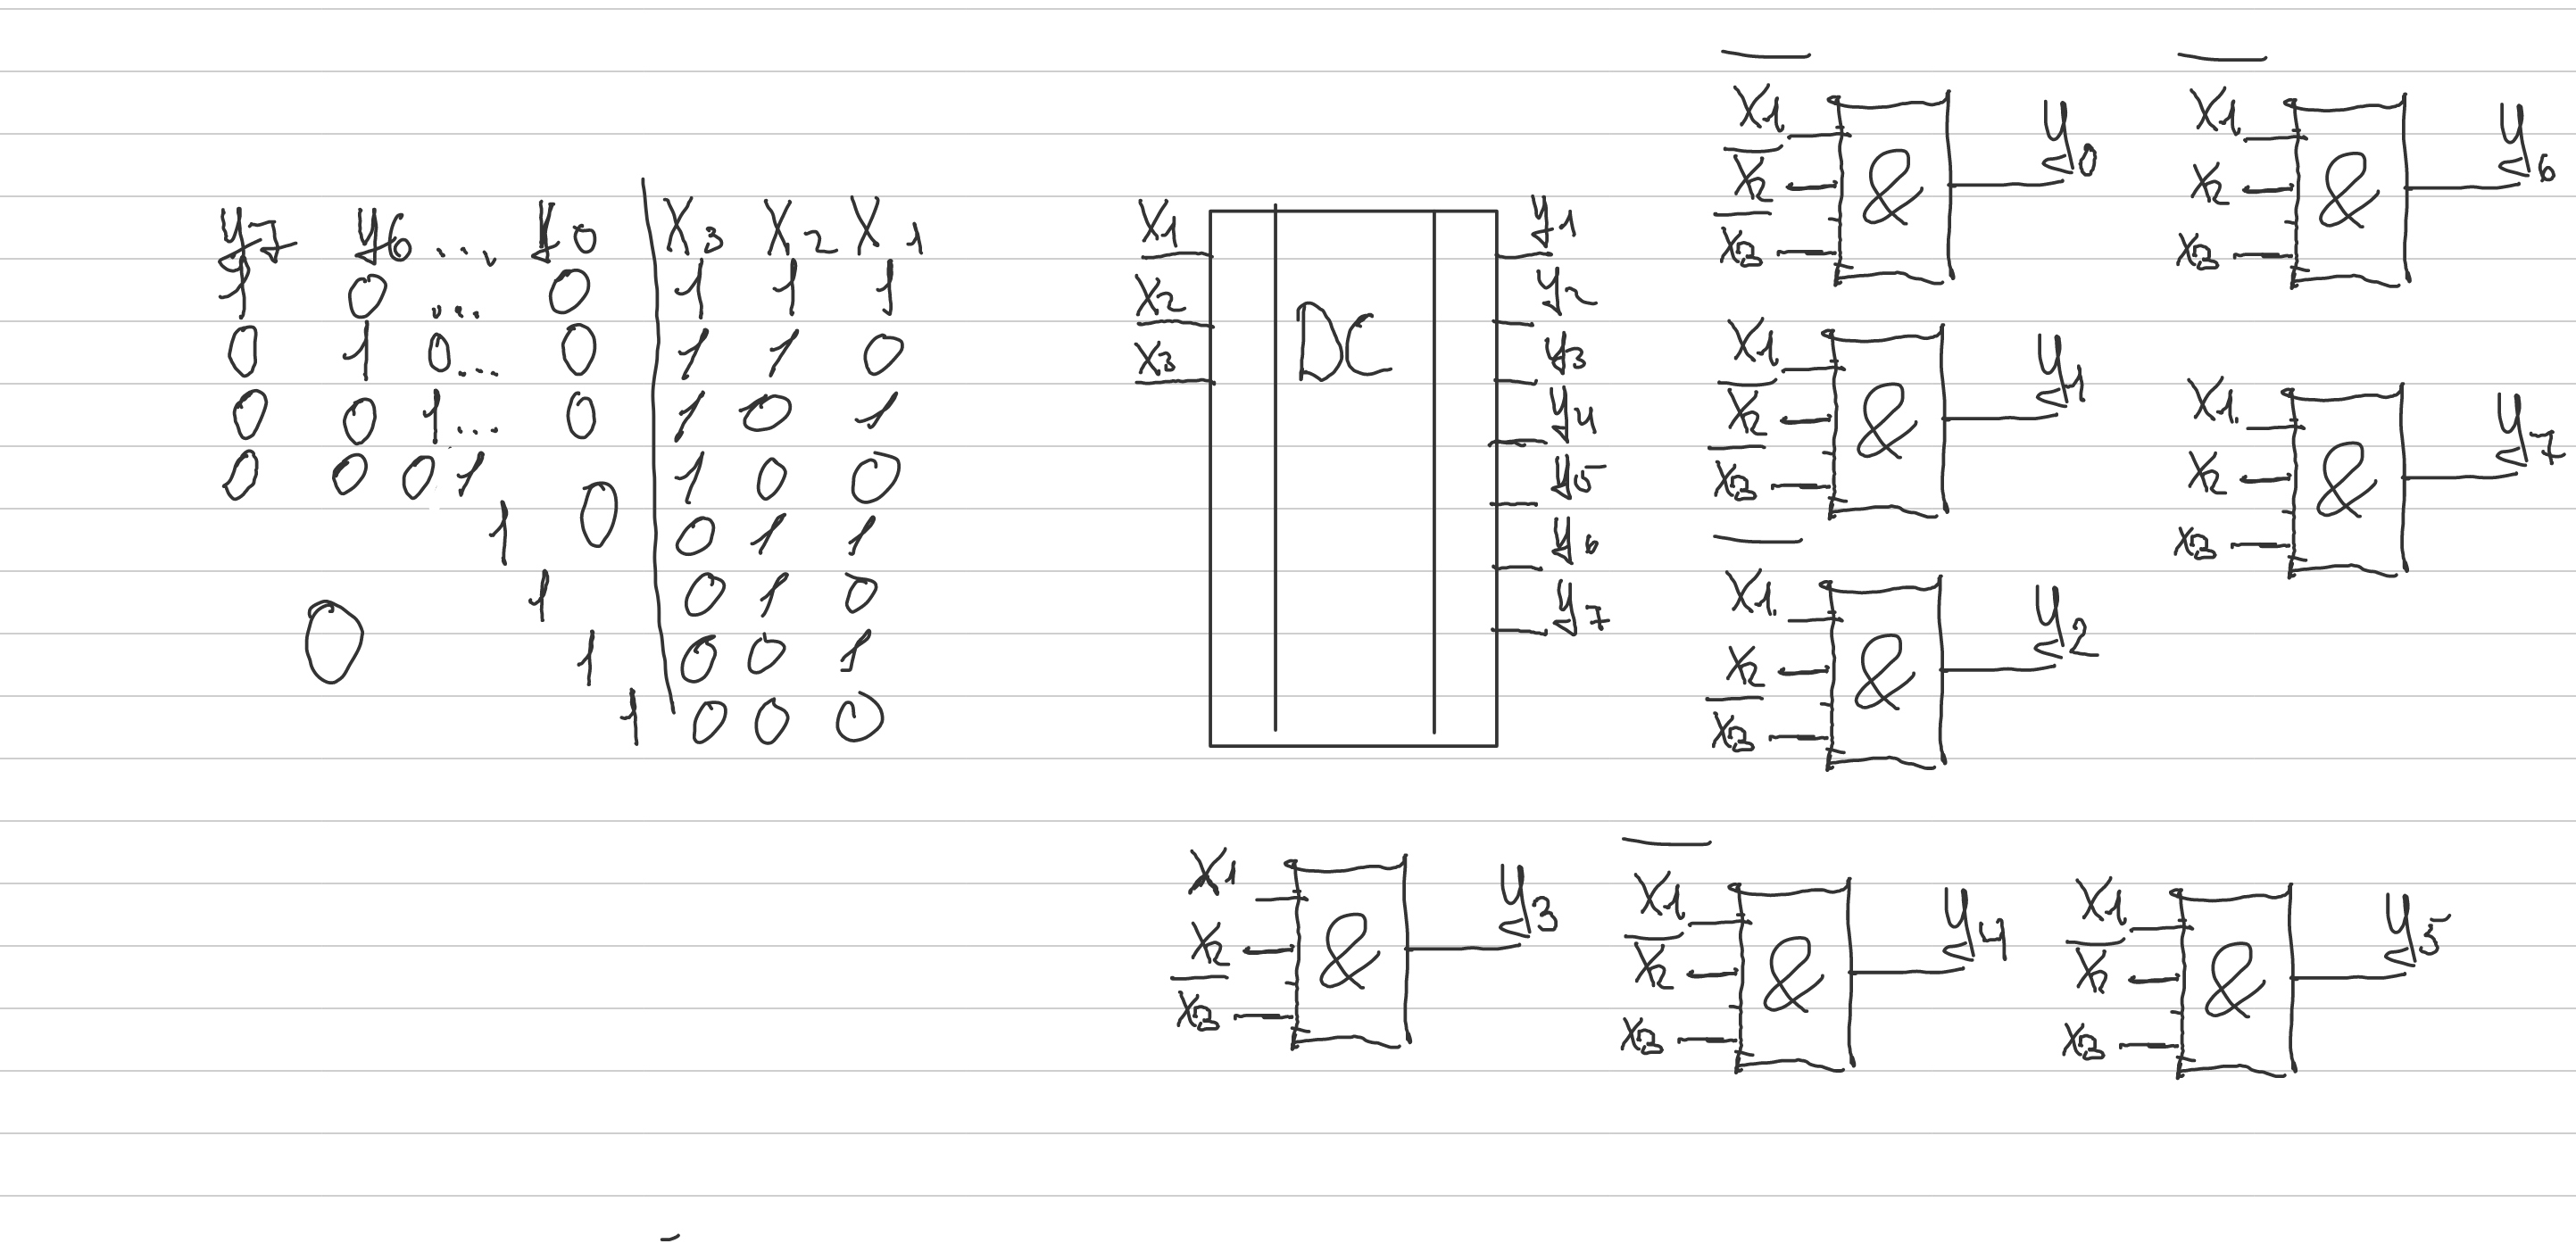
\includegraphics[width=\textwidth]{assets/decoder.png}

\hfill

Ниже приведено обозначение микросхемы К155ИД4

\hfill

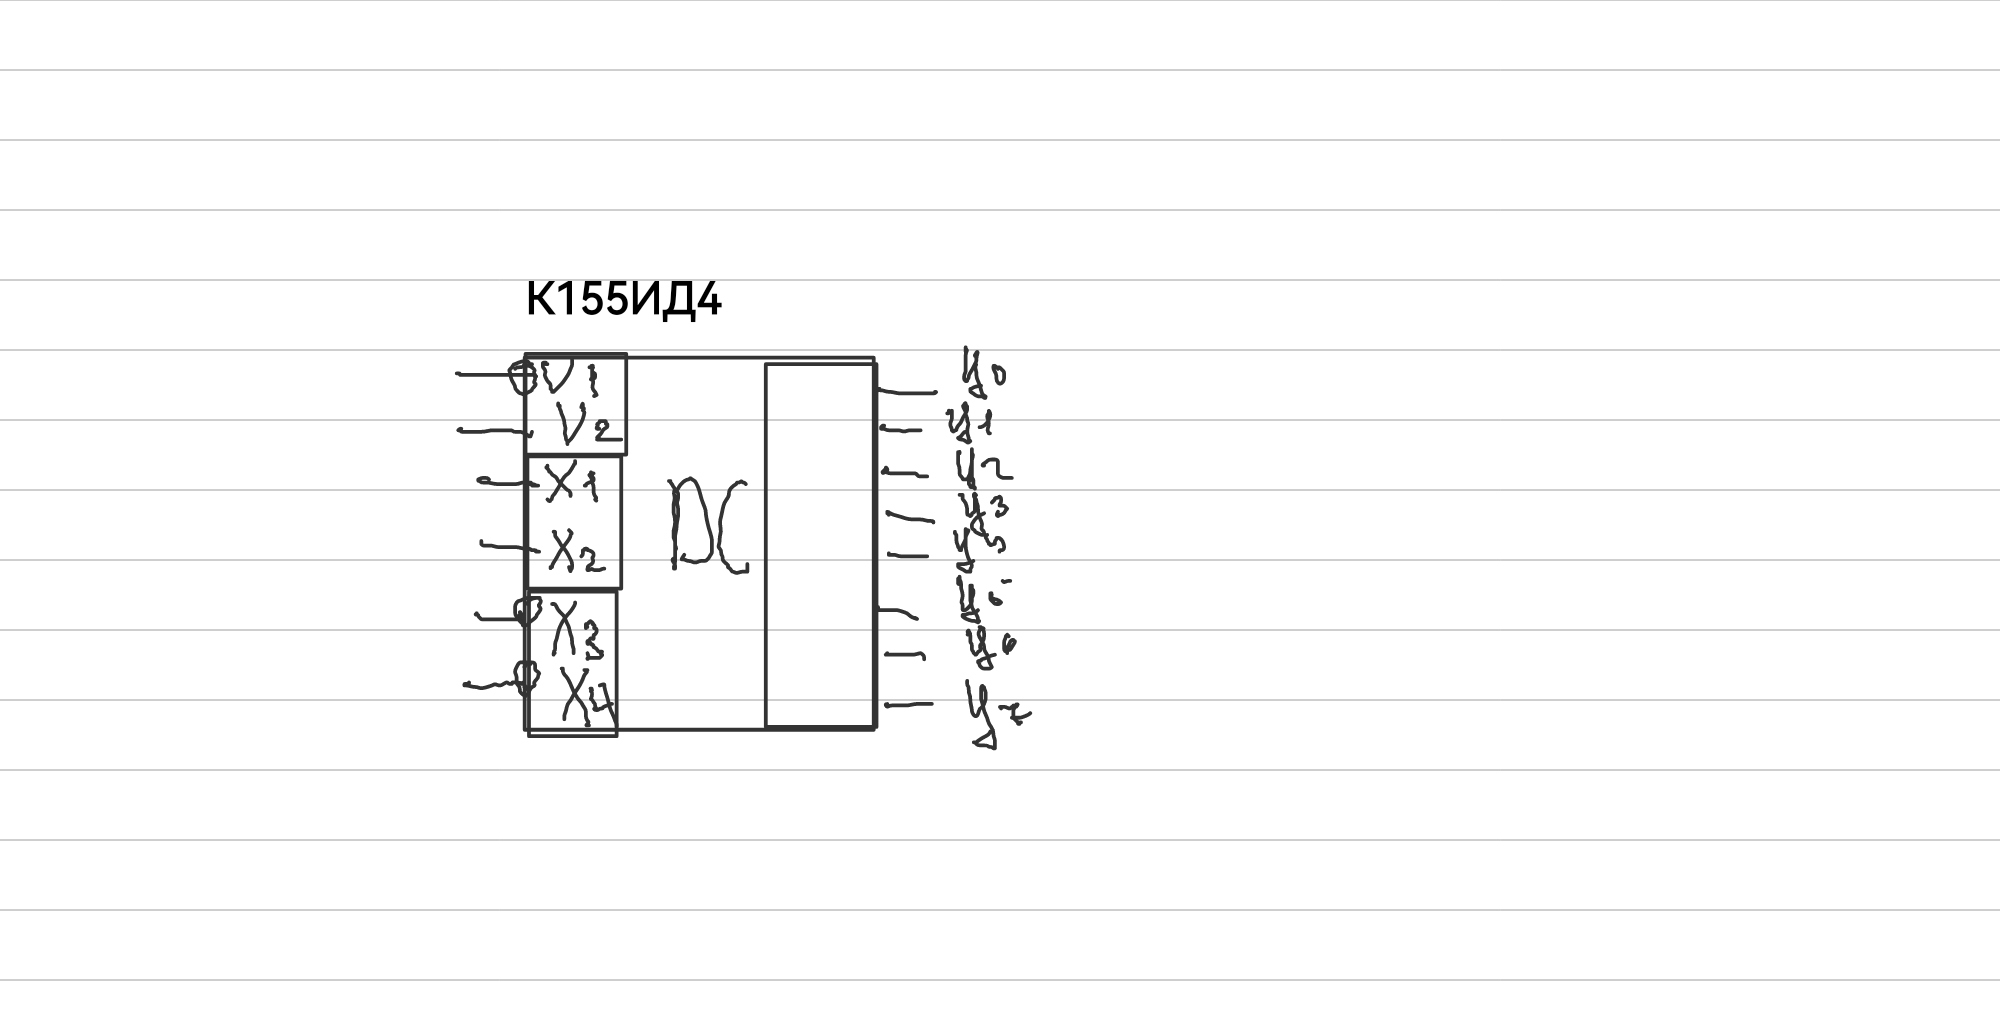
\includegraphics[width=\textwidth]{assets/k155id4.png}

Существуют также пирамидальные, каскадные дешифраторы.

\subsubsection{Каскадный дешифратор}

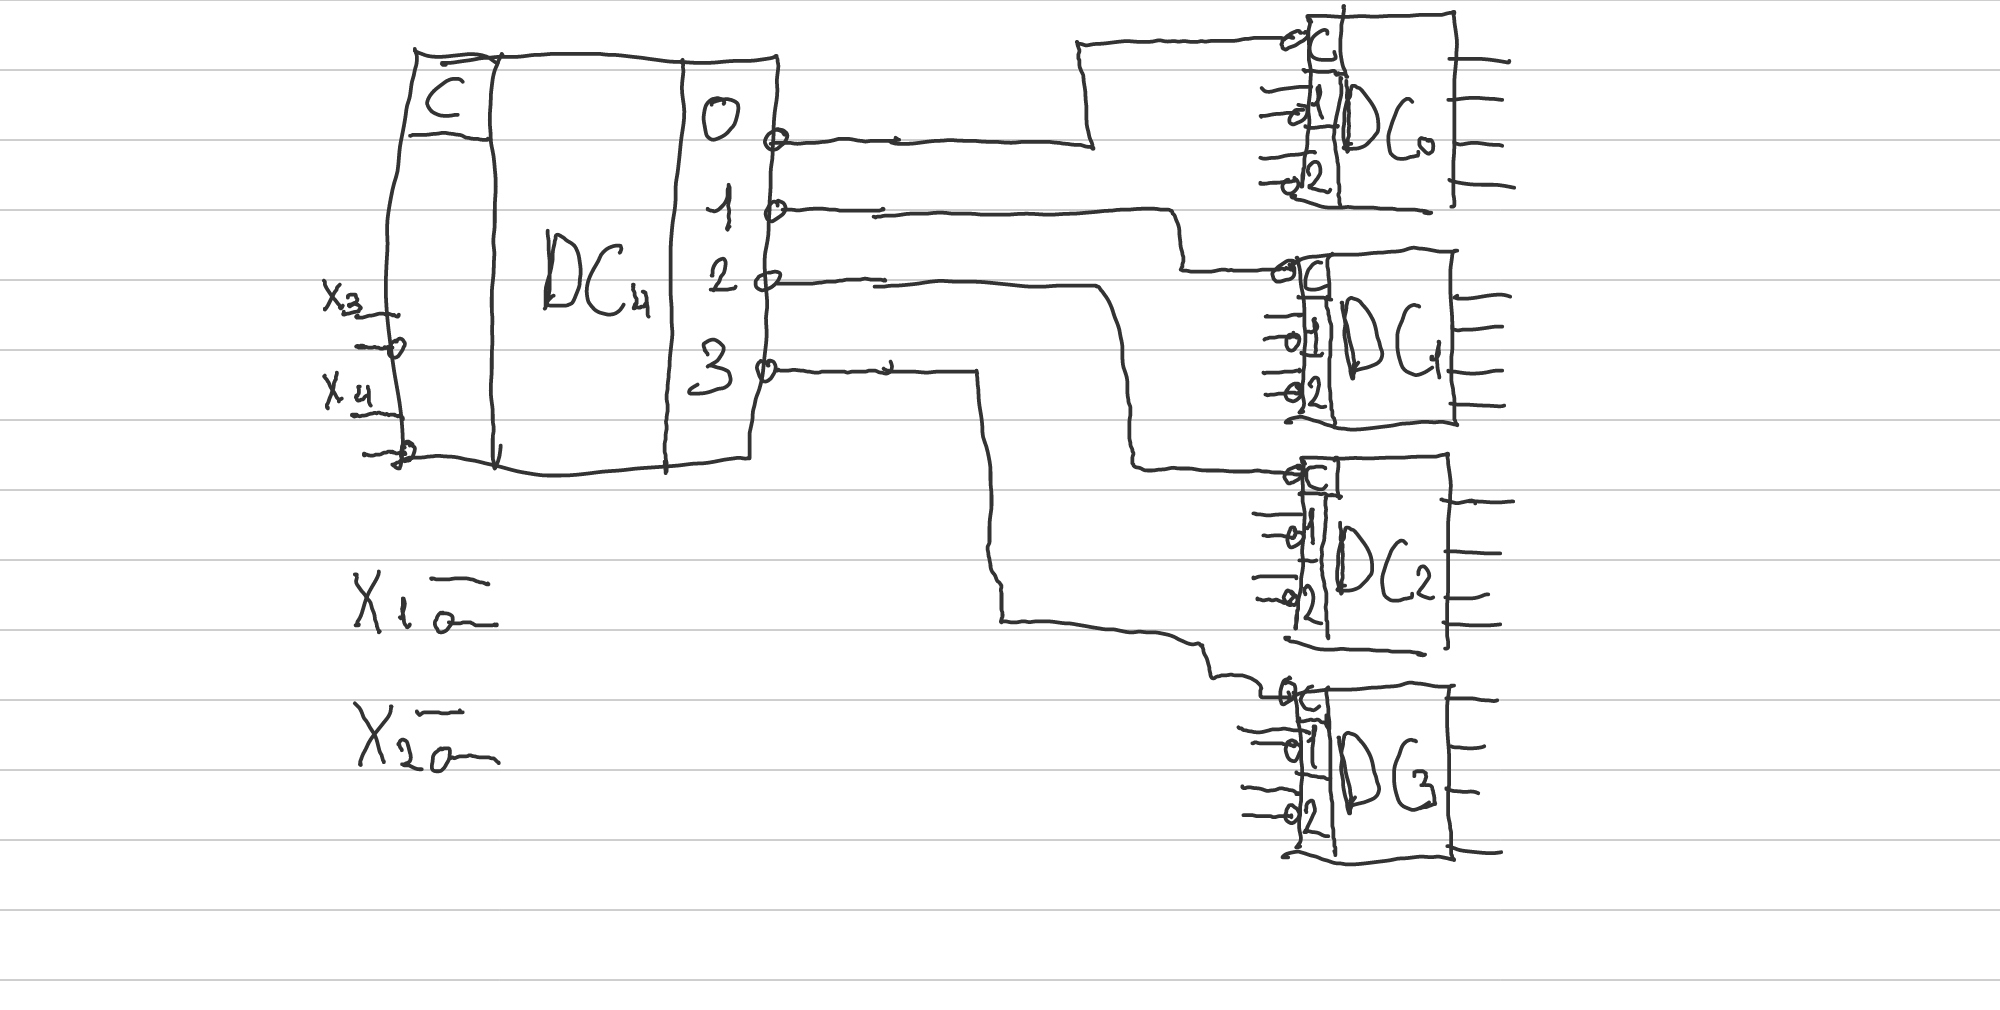
\includegraphics[width=\textwidth]{assets/cascade.png}

\subsection{Мультплексор}

Мультиплексор обеспечивает коммутацию на вход одного из входных сигналов.

Формула:

$y = \overline{x_3}\overline{x_2}\overline{x_1}D_0 + \overline{x_3}\overline{x_2}x_1D_1 + \overline{x_3}x_2\overline{x_1}D_2 + ... + x_3x_2x_1D_7$

\hfill

В формулу может быть добавлен управляющий сигнал:

$y = \overline{x_3}\overline{x_2}\overline{x_1}D_0\overline{v} + \overline{x_3}\overline{x_2}x_1D_1\overline{v} + \overline{x_3}x_2\overline{x_1}D_2\overline{v} + ... + x_3x_2x_1D_7\overline{v}$

\subsubsection{Схема}

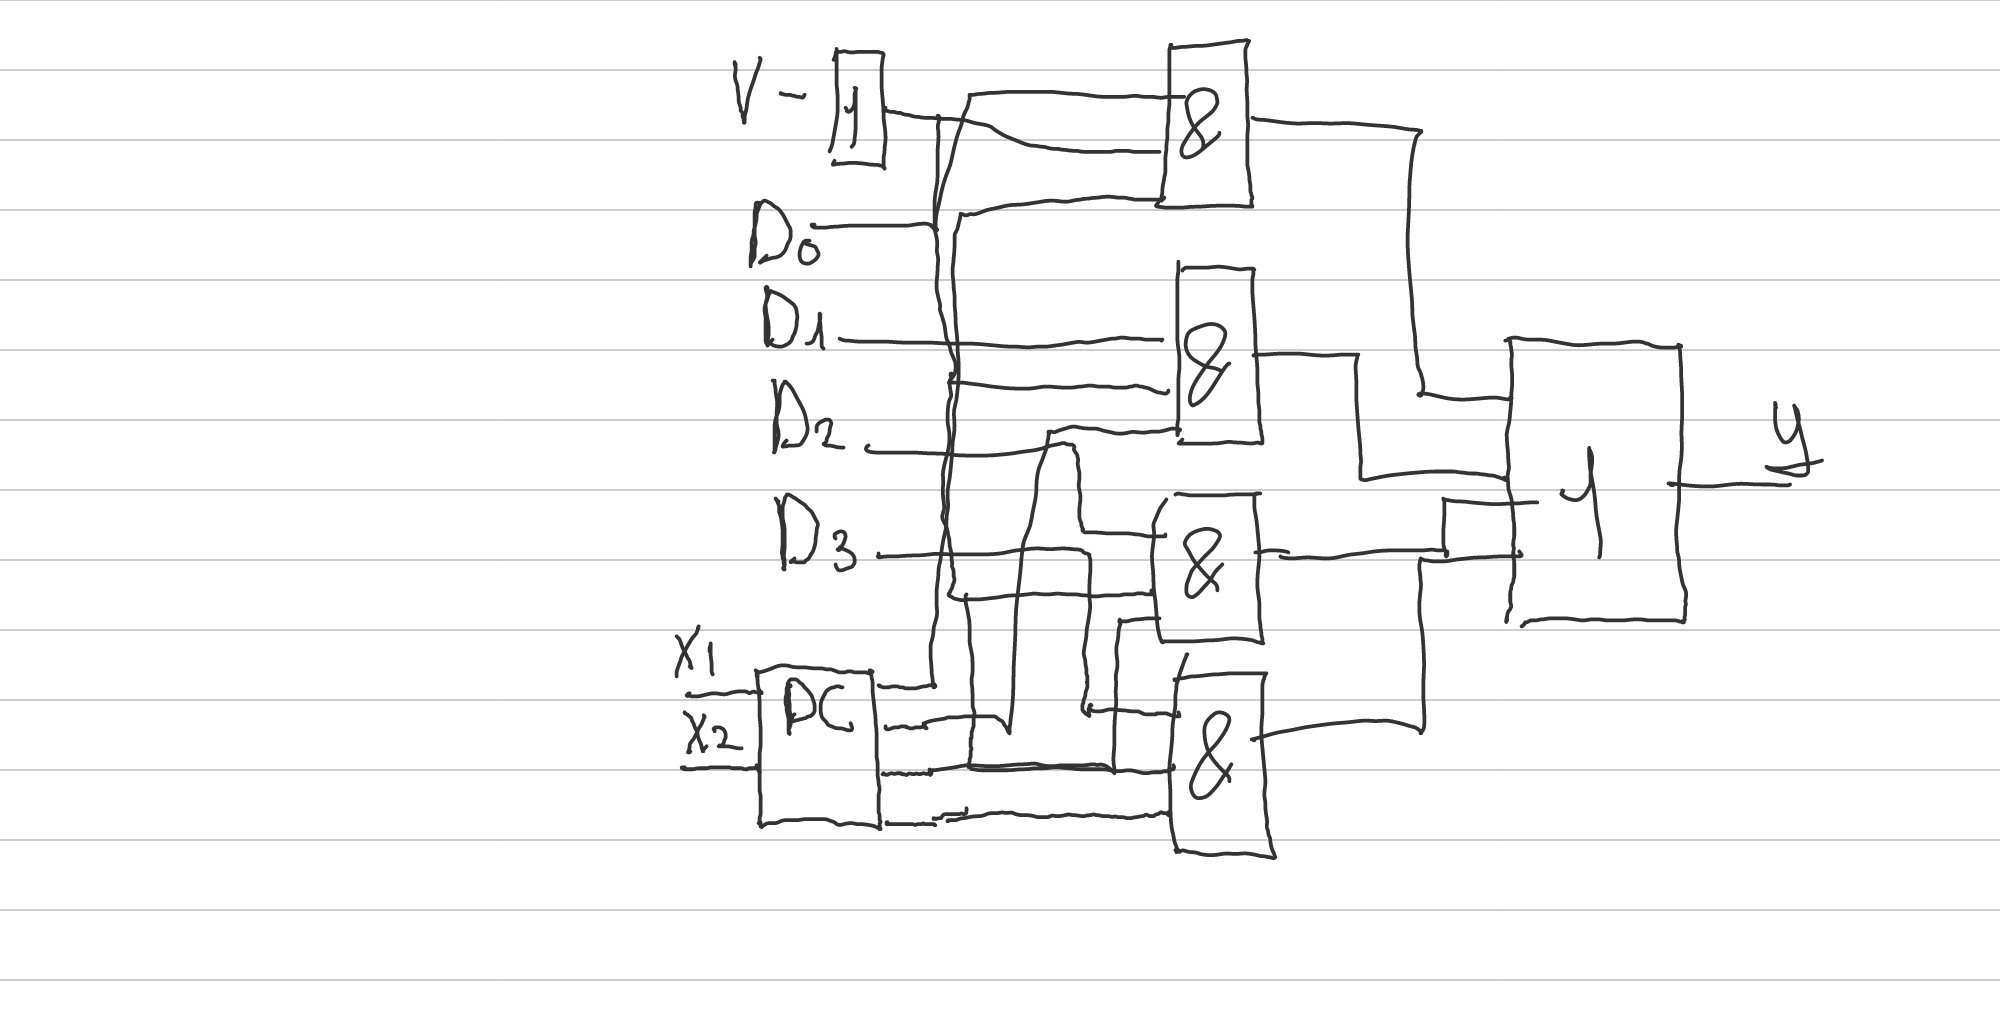
\includegraphics[width=\textwidth]{assets/multiplexer.png}

\subsubsection{Схема в multisim}

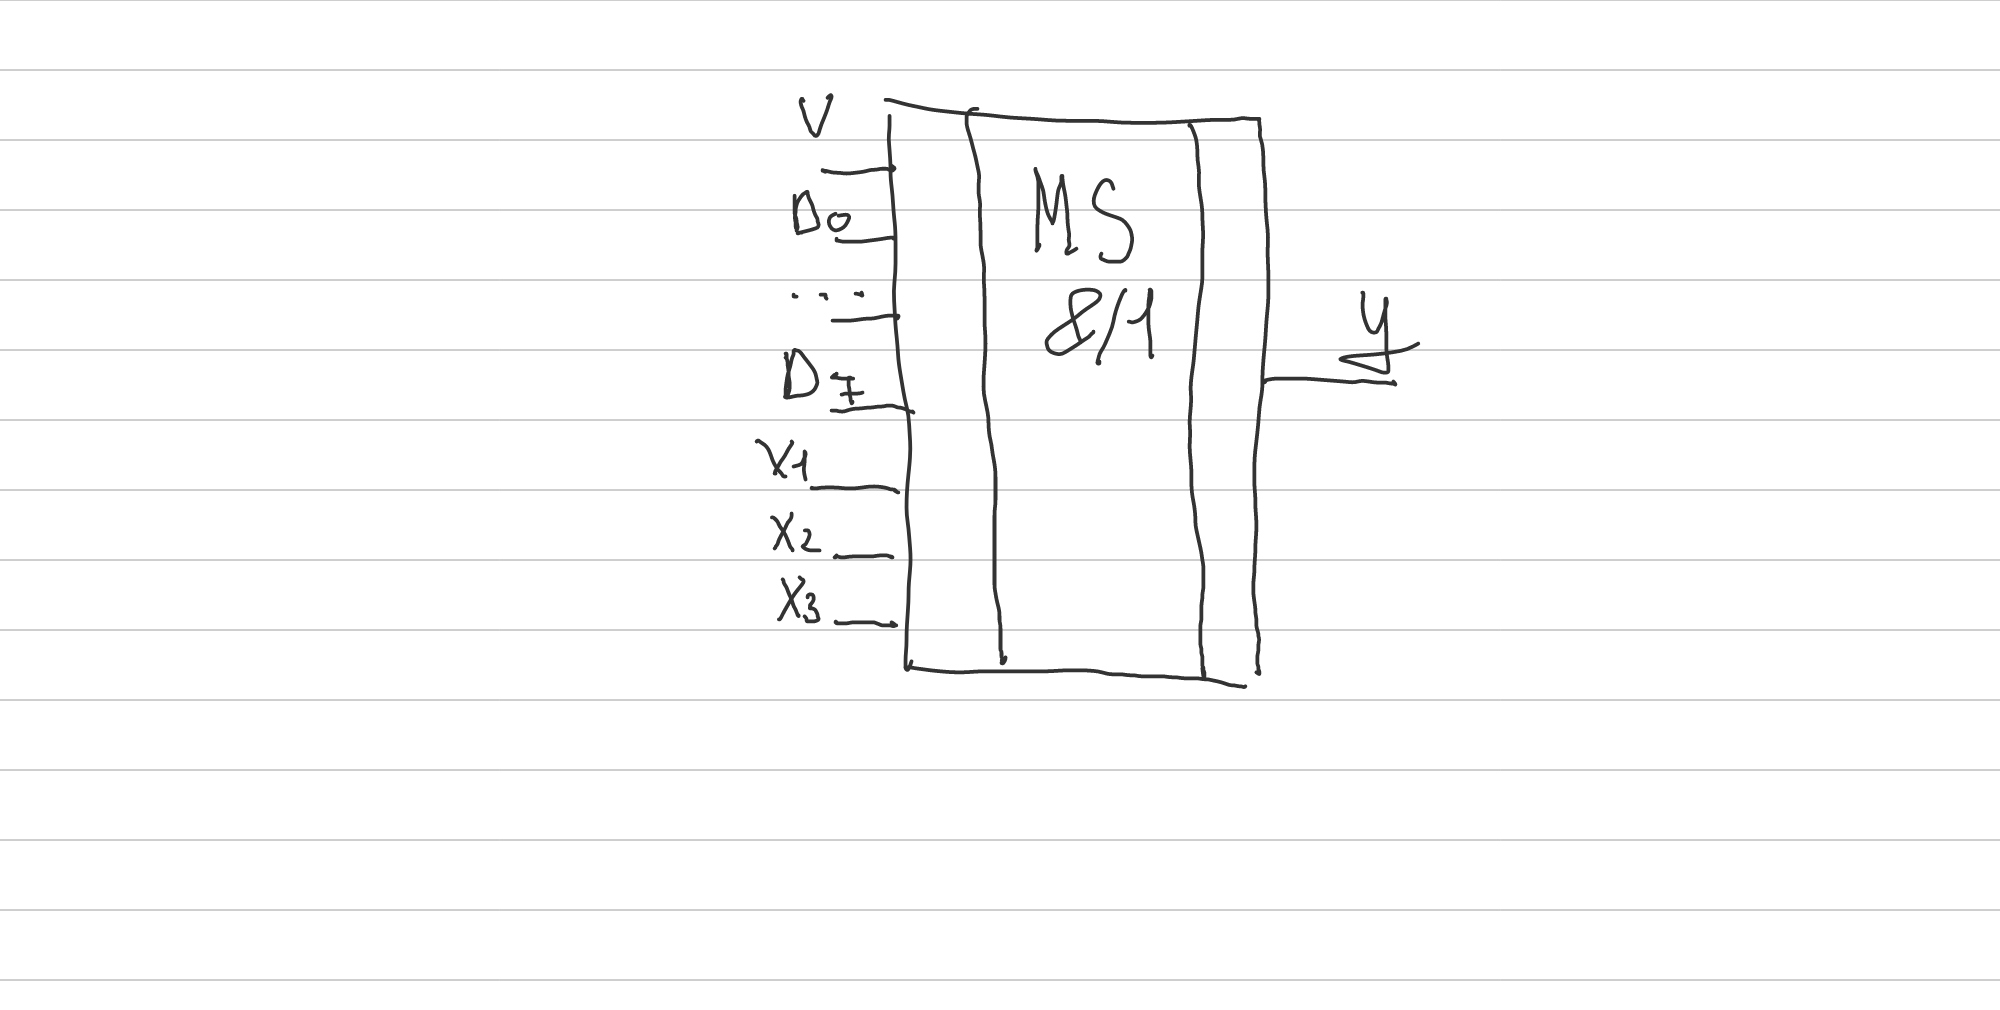
\includegraphics[width=\textwidth]{assets/multiplexer-multisim.png}

\subsection{Демультиплексор}

Демультиплексор — это логическое устройство, предназначенное для переключения сигнала с одного информационного входа на один из информационных выходов.

\hfill

Формула:

$y_0 = \overline{x_2} \overline{x_1} D, y_1 = \overline{x_1}D, y_2 = x_2\overline{x_1}D, y_3 = x_2 x_1 D$

\subsubsection{Схема}

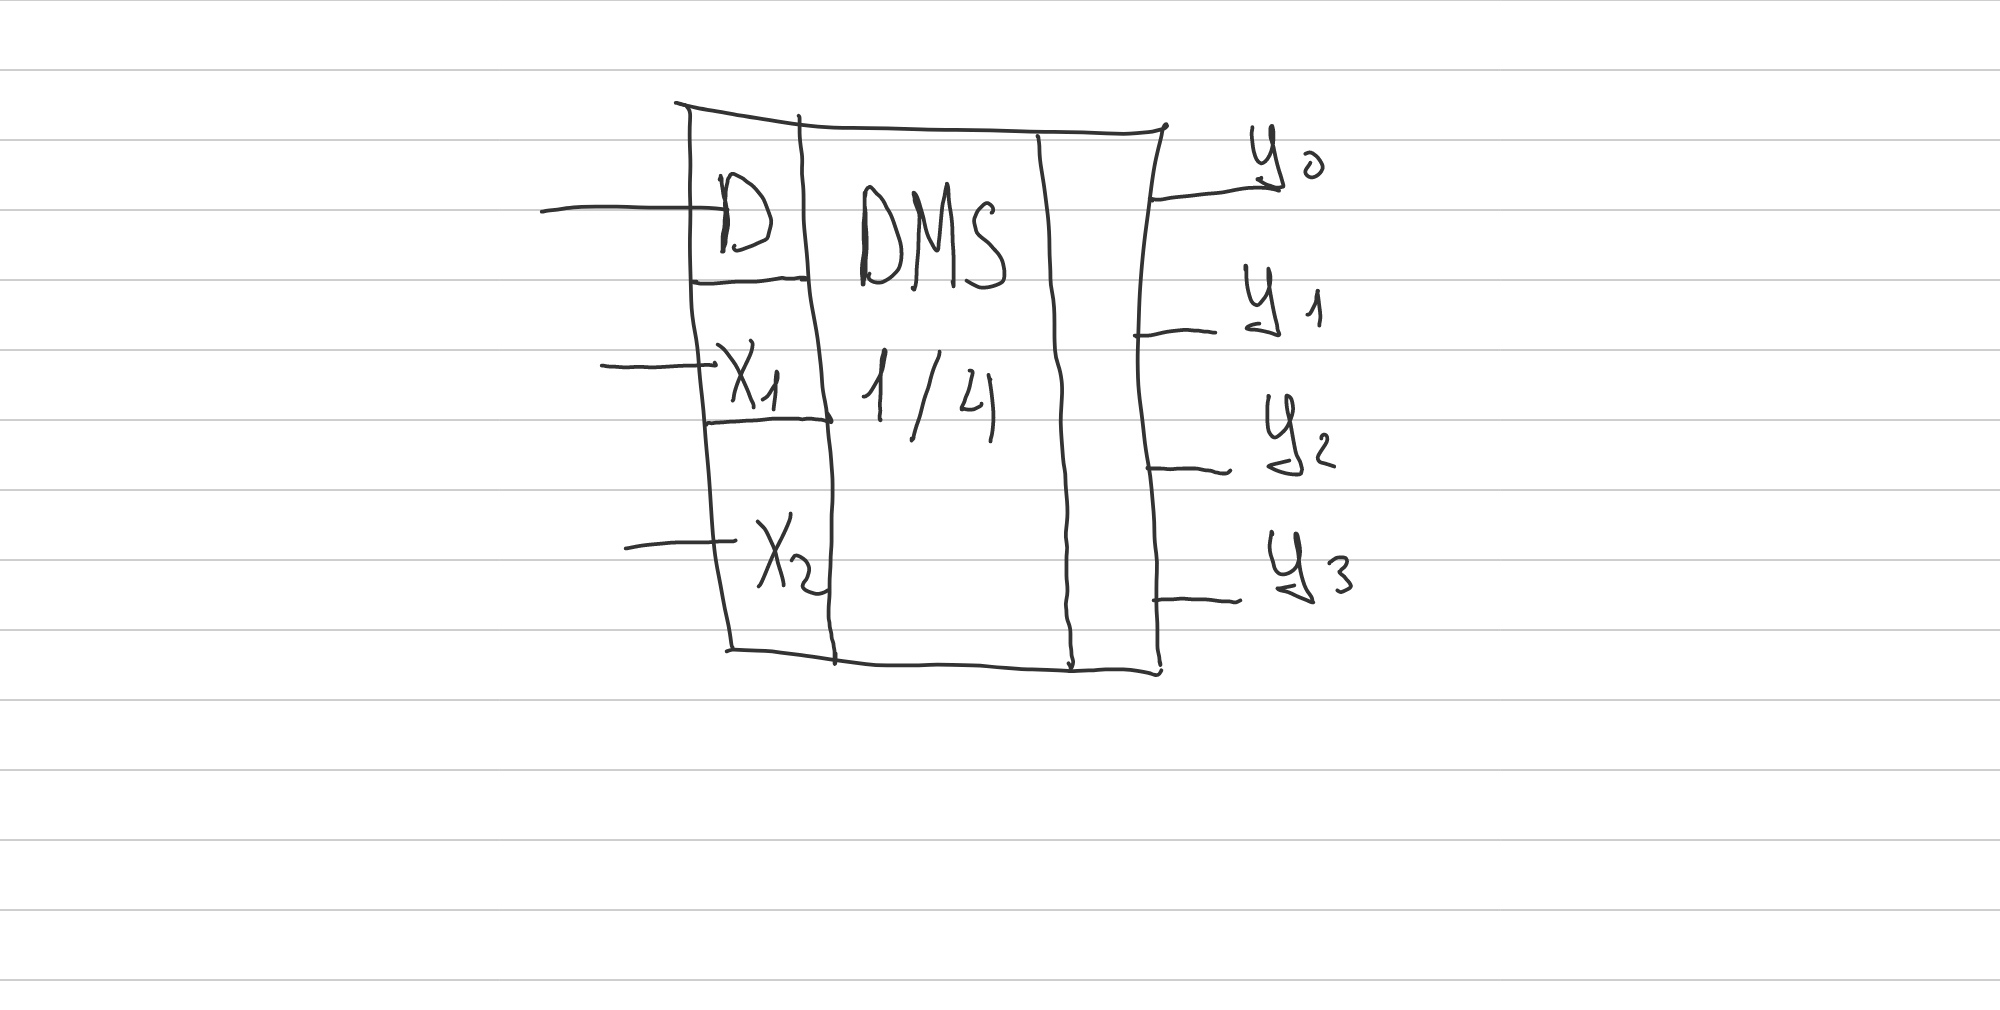
\includegraphics[width=\textwidth]{assets/demultiplexer.png}

\pagebreak
\section{Вычислительная техника - 17.10.2022}

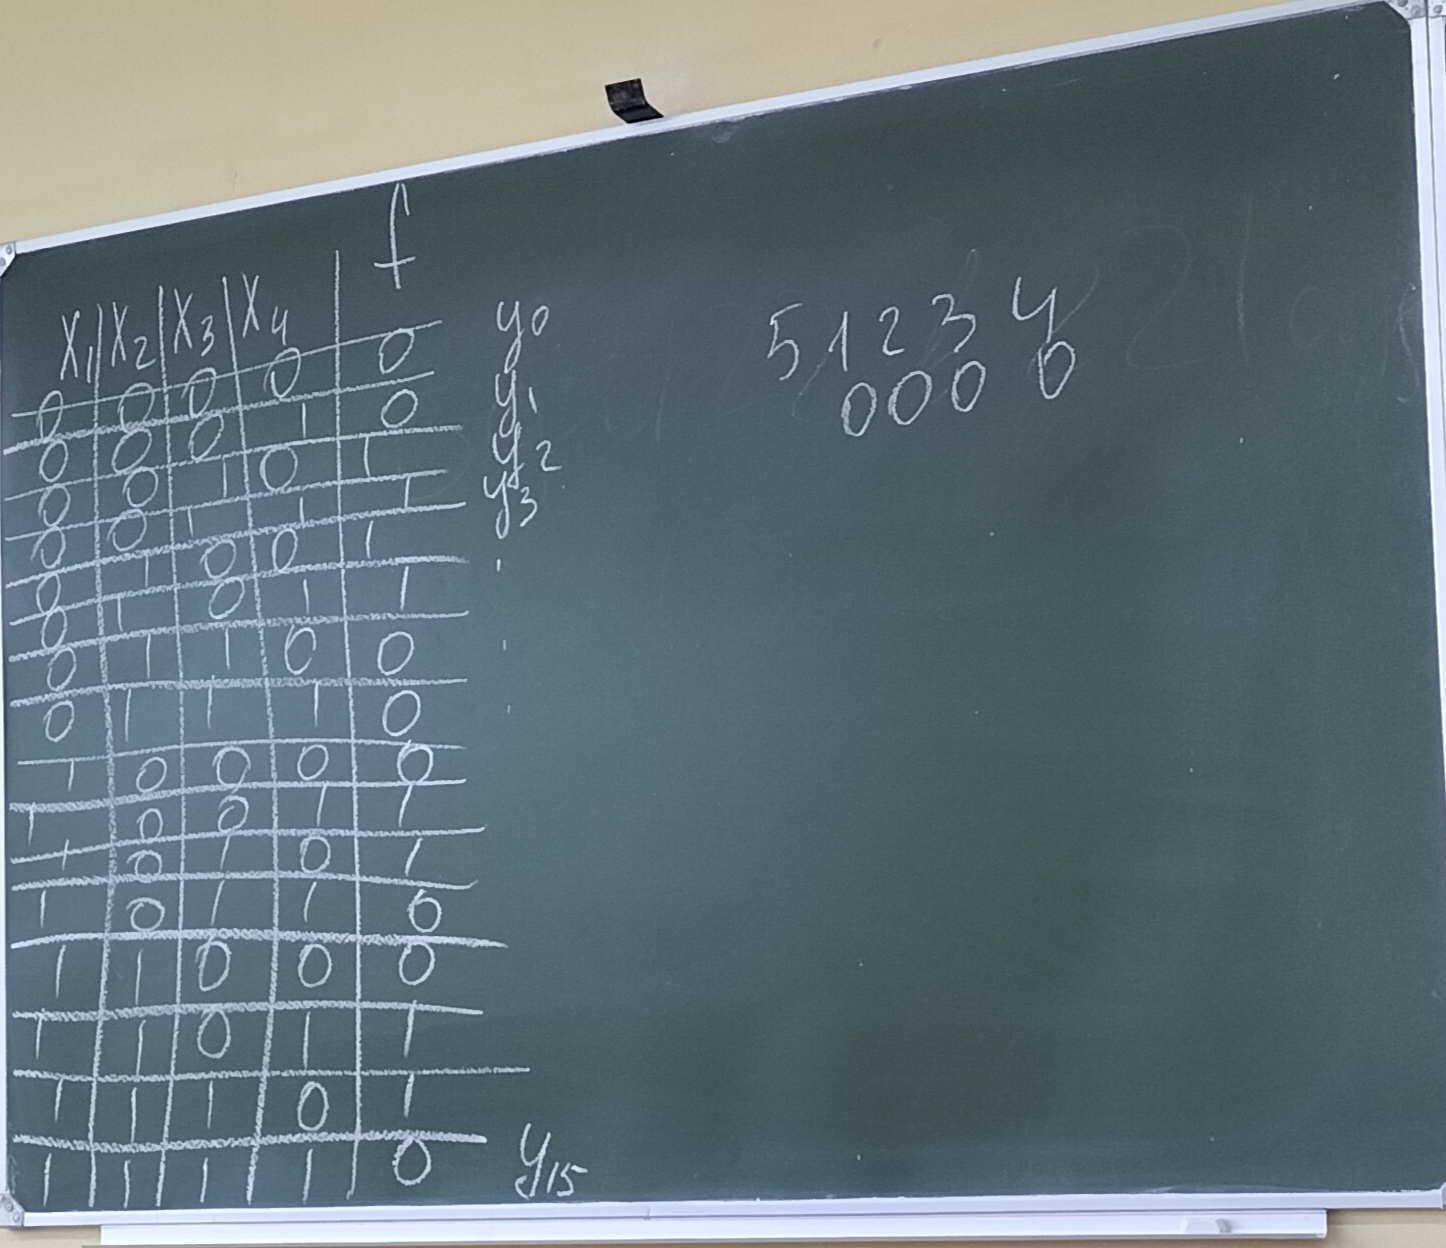
\includegraphics[width=\textwidth]{assets/image_1.jpg}

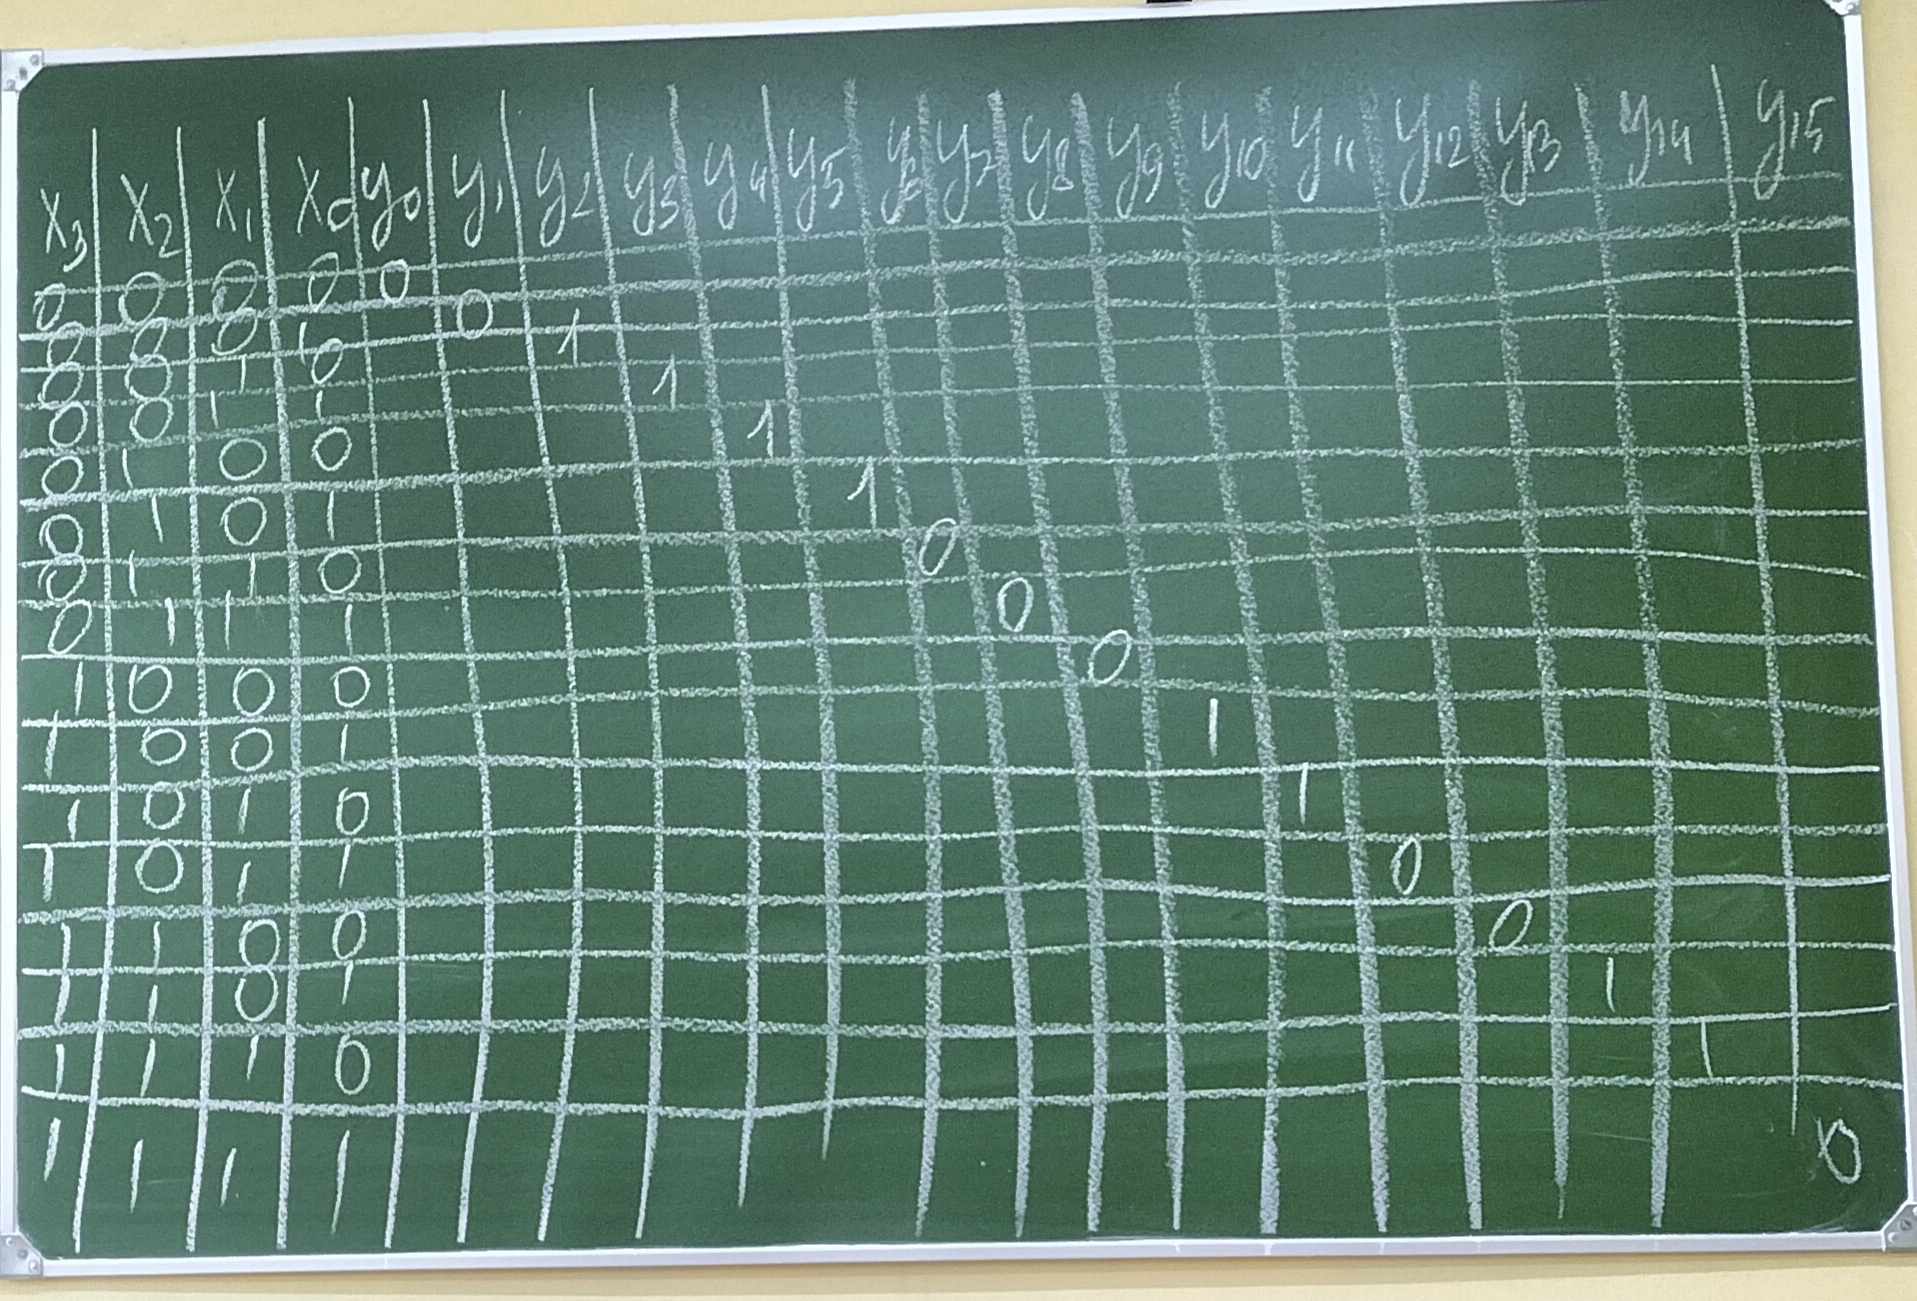
\includegraphics[width=\textwidth]{assets/image_2.jpg}

Показать работоспособность - попереключать ключики - показать, что лампчка зажигается.

\end{flushleft}

\end{document}
